% !TeX root = ../tfg.tex
% !TeX encoding = utf8

\chapter{Optimización y convexidad} \label{chap:optimizacion}

En el contexto del aprendizaje automático, la optimización constituye una herramienta fundamental para minimizar funciones de pérdida y estimar parámetros de forma eficiente.

En este capítulo se presentan los conceptos esenciales de optimización y convexidad, que permiten garantizar la existencia y unicidad de soluciones bajo ciertas condiciones. Se estudian preliminares como el teorema de la proyección convexa y se introducen algoritmos basados en gradientes, que constituyen la base de los métodos de entrenamiento en los modelos que se abordarán en los capítulos posteriores.



\section{Preliminares}
Comenzamos con el teorema de la proyección convexa. Este teorema nos va a proporcionar una propiedad muy relevante sobre los conjuntos convexos, ampliamente utilizados en problemas de optimización.

\begin{teorema}[Teorema de la proyección convexa] 
Sea $X \subset \mathbb{R}^n$ convexo, no vacío y cerrado, y sea $y \in \mathbb{R}^n$. Entonces existe un único $\bar{x} \in X$ tal que $\|y - \bar{x}\| \leq \|y - x\|,\ \forall x \in X$. \label{teo:proyeccion-convexa}
\end{teorema}

\vspace{0.2cm}

\textit{Dem.} Sea $r > 0$ tal que $A := \overline{B}(y,r) \cap X$ no sea vacío. Nótese que $A$ es compacto por ser la intersección de un conjunto compacto y uno cerrado. Entonces la función $d_y$ definida por $d_y(x) = \|x - y\|$ alcanza su mínimo en $A$, ya que es una función continua; es decir, existe $\bar{x} \in A$ tal que $d_y(\bar{x}) \leq d_y(x)$ para todo $x \in A$.

\vspace{0.2cm}

Además, $\bar{x}$ es el mínimo de $d_y$ en $X$, pues si $x \in X \setminus \overline{B}(y,r)$ se tiene que $\|x - y\| > r \geq \|y - \bar{x}\|$.

\vspace{0.2cm}

Para demostrar la unicidad, supongamos que existen dos puntos $x_1, x_2$ de proyección de $y$. Por la convexidad de $X$, el punto medio $x = \frac{x_1 + x_2}{2}$ del segmento entre ellos también pertenece a $X$. Ahora, dado que $d_y(x_1) = d_y(x_2)$:

\[
\frac{1}{2} \langle x_1 - x_2, y - x \rangle = \frac{1}{2} \left\langle x_1 - x_2, y - \frac{1}{2}(x_1 + x_2) \right\rangle
\]
\[
= \frac{1}{4} \langle (y - x_2) - (y - x_1), (y - x_1) + (y - x_2) \rangle
\]
\[
= \frac{1}{4} \left( \|y - x_1\|^2 - \|y - x_2\|^2 \right) = 0
\]

\vspace{0.2cm}

Por el teorema de Pitágoras se verifica que $\|y - x\|^2 + \left\|\frac{x_1 - x_2}{2}\right\|^2 = \|y - x_2\|^2$ y teniendo en cuenta que $x - x_2 = \frac{x_1 - x_2}{2}$ se obtiene la igualdad

\[
\|y - x\|^2 + \|x - x_2\|^2 = \|y - x_2\|^2
\]

\vspace{0.2cm}

de modo que $\|y - x\|^2 \leq \|y - x_2\|^2$. La igualdad se da si, y solo si, $x = x_2$, por lo que $x_1 = x_2$. \hfill $\Box$

Este $\bar{x}$ se llama \textit{proyección convexa} de $y$ sobre $X$ y se denotará por $P_X(y)$.



\section{Algoritmos de optimización basados en gradientes}
La mayoría de los algoritmos de aprendizaje implican algún tipo de optimización. La optimización se refiere a la tarea de minimizar o maximizar alguna función $f(x)$ mediante la alteración de $x$. Solemos plantear la mayoría de los problemas de optimización en términos de minimización de $f(x)$. La maximización puede lograrse mediante un algoritmo de minimización minimizando $-f(x)$.

La función que queremos minimizar o maximizar se llama función objetivo o criterio. Cuando la estamos minimizando, también podemos llamarla función de coste, función de pérdida o función de error. 

A menudo denotamos el valor que minimiza (o maximiza) la función con un superíndice *. Por ejemplo:

\[
x^* = \arg\min_x f(x).
\]

Es habitual trabajar con funciones objetivo diferenciables y aprovechar las propiedades del gradiente para optimizar el valor de la función objetivo. A continuación se describe la base fundamental de estos métodos: el gradiente descendente. También se discute cómo optimizar funciones definidas en conjuntos con restricciones convexas.

\subsection{Descenso de gradiente}
Es conocido que el gradiente de una función diferenciable tiene la dirección de la máxima pendiente en el grafo de la función, por lo que avanzando pequeñas cantidades en la dirección opuesta a la del gradiente conseguimos reducir el valor de la función. Este método iterativo es el que se conoce como gradiente descendente.

Analicemos más en profundidad el gradiente descendente, un método clásico para la minimización de funciones. 

La regla de actualización de este método iterativo, para encontrar un $x \in \mathbb{R}^d$ que minimice una función objetivo diferenciable $f : \mathbb{R}^d \to \mathbb{R}$ viene dada por 
\[
x_{t+1} = x_t - \eta \nabla f(x_t), \quad t \in \mathbb{N} \cup \{0\},
\]
donde $\eta$ es la cantidad que se avanza en la dirección del gradiente, y se denomina tasa de aprendizaje. Dicho $\eta$ puede ser constante o puede ir adaptándose de acuerdo con las evaluaciones de la función objetivo. En el primer caso, la elección de un $\eta$ demasiado grande o demasiado pequeño puede conducir a malos resultados. El segundo caso requiere evaluar la función objetivo en cada iteración, lo que puede ser costoso computacionalmente.

\vspace{0.3cm}

Los fundamentos del gradiente descendente se basan en las siguientes ideas. Consideramos una función objetivo $f : \mathbb{R}^d \to \mathbb{R}$, $x \in \Omega$ y $v \in \mathbb{R}^d \setminus \{0\}$ una dirección arbitraria. Consideramos la función $g: \mathbb{R} \to \mathbb{R}$ dada por 
\[
g(\eta) = f(x + \eta \frac{v}{\|v\|}).
\]
La tasa de variación o derivada direccional de $f$ en $x$ para la dirección $v$ viene dada por 
\[
g'(0) = \frac{1}{\|v\|} \langle \nabla f(x), v \rangle.
\]
Aplicando la desigualdad de Cauchy-Schwarz, se tiene
\[
- \|\nabla f(x)\| \leq \frac{1}{\|v\|} \langle \nabla f(x), v \rangle \leq \|\nabla f(x)\|,
\]
y la igualdad en la desigualdad izquierda se alcanza cuando $v = -\nabla f(x)$, obteniendo así la tasa máxima de descenso. De la misma forma, la tasa de máximo ascenso se alcanza con $\nabla f(x)$.

\vspace{0.3cm}

Si el gradiente en $x$ es no nulo, y consideramos la aproximación de Taylor de primer orden para los puntos $x - \eta \nabla f(x)$, se tiene
\[
f(x - \eta \nabla f(x)) = f(x) - \eta \|\nabla f(x)\|^2 + o(\eta),
\]
con $\lim_{\eta \to 0} \frac{o(\eta)}{\eta} = 0$, luego existe $\varepsilon > 0$ tal que si $0 < \delta < \varepsilon$, se tiene
\[
\frac{o(\delta)}{\delta} < \|\nabla f(x)\|,
\]
y por tanto,
\[
f(x - \delta \nabla f(x)) - f(x) = \delta \left( -\|\nabla f(x)\|^2 + \frac{o(\delta)}{\delta} \right) < \delta \left( -\|\nabla f(x)\|^2 + \|\nabla f(x)\| \right) = 0.
\]

luego $f(x - \delta \nabla f(x)) < f(x)$ para $0 < \delta < \varepsilon$, luego tenemos garantizado que para una tasa de aprendizaje adecuada el método puede descender en cada iteración. 

Podemos observar que la dirección del gradiente no es la única dirección de descenso válida, sino que lo anterior sigue siendo válido para cualquier dirección $v \in \mathbb{R}^d$ con $\langle \nabla f(x), v \rangle < 0$. La elección de otras direcciones de descenso, aunque no sean las de máxima pendiente, pueden proporcionar mejores resultados en problemas determinados.

\vspace{0.3cm}

Cuando trabajamos con problemas de optimización con restricciones, el método del gradiente no puede ser aplicado directamente, pues la regla de adaptación $x_{t+1} = x_t - \eta \nabla f(x_t)$ no garantiza que $x_{t+1}$ sea un punto viable. El método del gradiente con proyecciones soluciona este problema, cuando el problema de optimización es convexo, añadiendo una proyección sobre el conjunto viable en la regla de adaptación, es decir, si $C$ es el conjunto convexo determinado por las restricciones (que supondremos también cerrado, esta condición se tiene cuando las funciones restricción son continuas, y la convexidad garantiza la continuidad en el interior del dominio), y $P_C$ es la proyección sobre dicho conjunto, entonces la regla de adaptación se convierte en
\[
x_{t+1} = P_C(x_t - \eta \nabla f(x_t)).
\]
Para confirmar la validez de este método, tenemos que ver que la dirección $v = P_C(x - \eta \nabla f(x)) - x$ es una dirección de descenso, lo cual, por lo razonado anteriormente, se consigue si $\langle \nabla f(x), v \rangle < 0$.

\vspace{0.3cm}

Llamamos $x_1 = x - \eta \nabla f(x)$. Entonces, $v = P_C(x_1) - x$. Notemos que $\langle \nabla f(x), v \rangle < 0 \implies \langle x - x_1, P_C(x_1) - x \rangle = -\eta \langle \nabla f(x), v \rangle > 0$. Si el gradiente es no nulo y $x_1 \in C$, entonces $\langle x - x_1, x - x_1 \rangle = \|x_1 - x\|^2 > 0$. 

Si $x_1 \notin C$, entonces el teorema de la proyección convexa \ref{teo:proyeccion-convexa} asegura que el semiespacio 
\[
H = \{ y \in \mathbb{R}^d : \langle x_1 - P_C(x_1), y - P_C(x_1) \rangle \leq 0 \}
\]
contiene a $C$. En particular,
\[
0 \geq \langle x_1 - P_C(x_1), x - P_C(x_1) \rangle = \langle x_1 - x, x - P_C(x_1) \rangle + \|x - P_C(x_1)\|^2.
\]

\vspace{0.3cm}

En consecuencia, $\langle x_1 - x, P_C(x_1) - x \rangle \geq \|x - P_C(x_1)\|^2 \geq 0$. Además, la igualdad se da si y solo si $x = P_C(x_1)$, y en tal caso el algoritmo habrá convergido (observemos que esto ocurre cuando $x \in \text{Fr } C$ y la dirección de descenso proporcionada por el gradiente apunta hacia fuera de $C$ y de forma ortogonal al hiperplano soporte). Por tanto, mientras las iteraciones del gradiente con proyecciones provoquen algún movimiento en los puntos obtenidos, escogiendo la tasa de aprendizaje adecuada, tenemos la garantía de poder descender en la función objetivo.  En la Figura \ref{fig:convergencia} se pueden comparar visualmente el gradiente con proyecciones y el gradiente descendente.

\begin{figure}[!htbp]
    \centering
    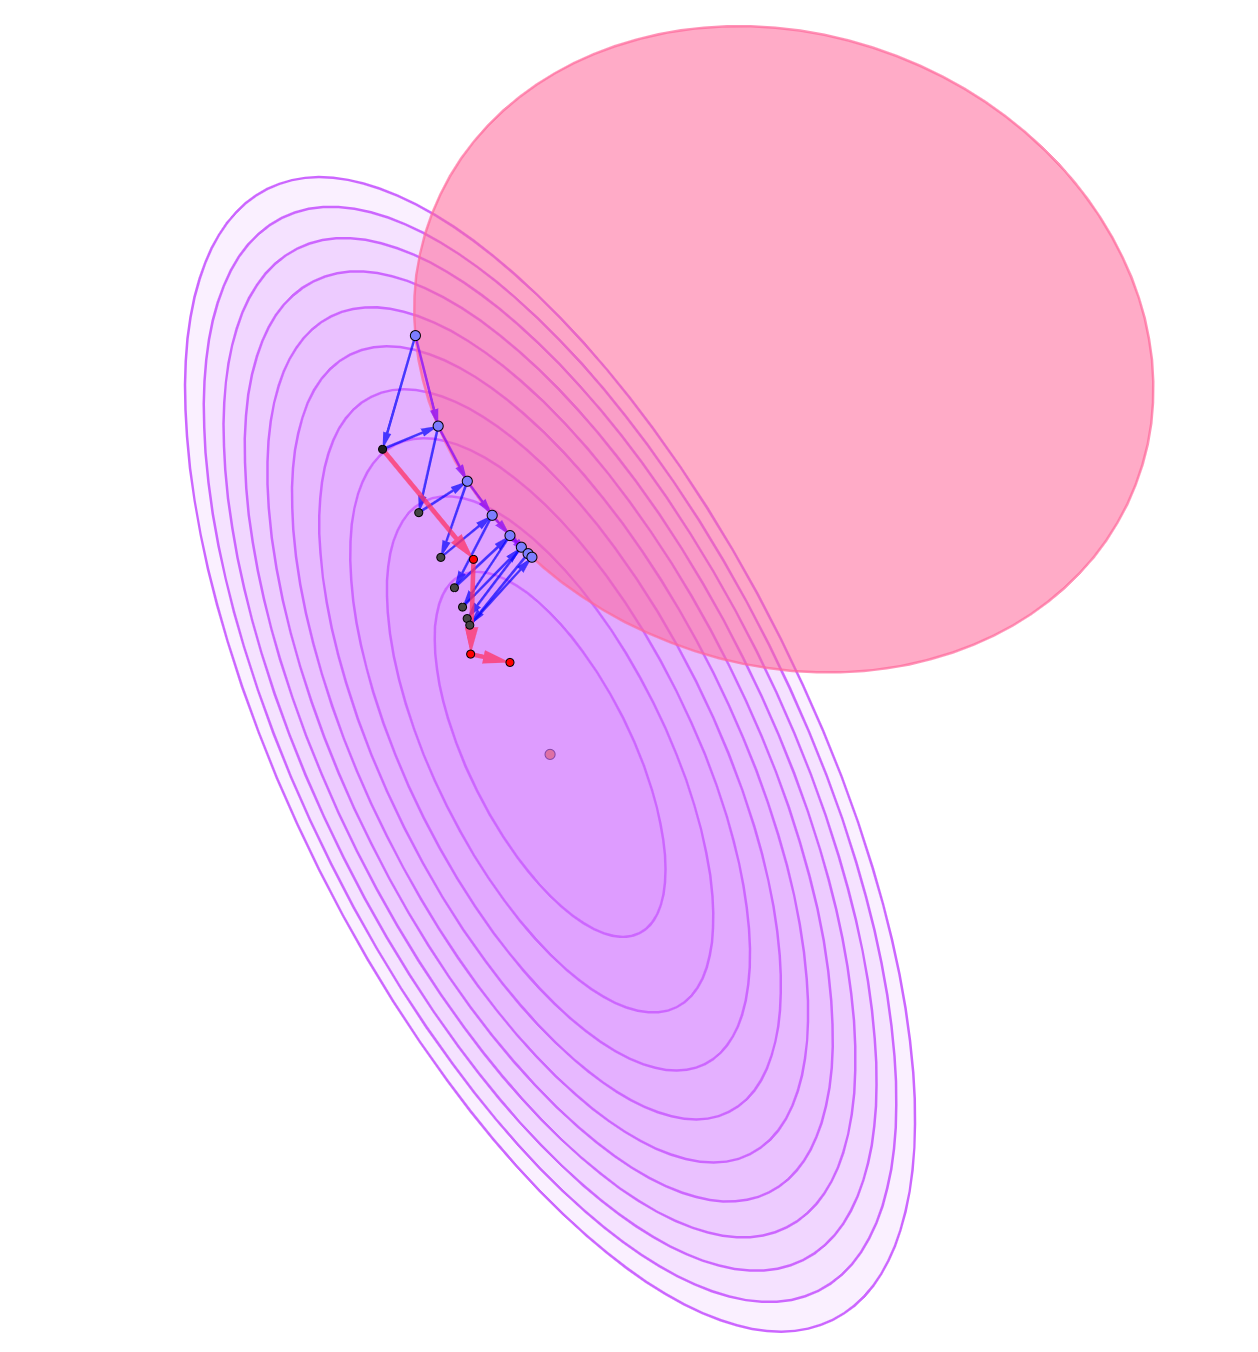
\includegraphics[width=0.8\textwidth]{img/convergencia.png}
    \caption{Curvas de nivel de una función objetivo a optimizar (morado). Gradiente descendente (recorrido rojo) y gradiente descendente con proyecciones sobre un conjunto convexo (azul). Se puede observar que el recorrido que se sigue sobre el conjunto convexo también minimiza la función objetivo.}
    \label{fig:convergencia}
\end{figure}

\subsection{Jacobiano y Hessiano}

Cuando la función tiene entradas y salidas vectoriales, usamos la \emph{matriz Jacobiana}. Para \( f : \mathbb{R}^n \to \mathbb{R}^m \), con \( f = (f_1, f_2, \ldots, f_m) \), el Jacobiano en un punto \( x \in \mathbb{R}^n \) se define como:

\[
J_f(x) = 
\begin{pmatrix}
\frac{\partial f_1}{\partial x_1}(x) & \frac{\partial f_1}{\partial x_2}(x) & \cdots & \frac{\partial f_1}{\partial x_n}(x) \\
\frac{\partial f_2}{\partial x_1}(x) & \frac{\partial f_2}{\partial x_2}(x) & \cdots & \frac{\partial f_2}{\partial x_n}(x) \\
\vdots & \vdots & \ddots & \vdots \\
\frac{\partial f_m}{\partial x_1}(x) & \frac{\partial f_m}{\partial x_2}(x) & \cdots & \frac{\partial f_m}{\partial x_n}(x)
\end{pmatrix}
=
\begin{pmatrix}
\nabla f_1(x) \\
\vdots \\
\nabla f_m(x)
\end{pmatrix},
\]

donde \(\nabla f_i(x)\) es el \emph{gradiente} de la i-ésima componente escalar.

La \emph{segunda derivada} o \emph{Hessiano} se usa para funciones \( f : \mathbb{R}^n \to \mathbb{R} \). Su definición es:

\[
H_{i,j} = \frac{\partial^2 f}{\partial x_i \partial x_j}.
\]

El Hessiano es \emph{simétrico} si las segundas derivadas son continuas.

\begin{itemize}
  \item Si el Hessiano es positivo definido, el punto es un mínimo local.
  \item Si es negativo definido es un máximo local.
  \item Si tiene valores propios positivos y negativos, es un punto de silla.
\end{itemize}


\subsubsection{Número de condición del Hessiano}
El \emph{número de condición} del Hessiano indica las diferencias entre las curvaturas en distintas direcciones. Un número de condición alto dificulta el descenso por gradiente porque en una dirección la derivada puede crecer rápido yn otra dirección puede crecer lento. Esto obliga a elegir tasas de aprendizaje pequeñas, ralentizando la convergencia.

\subsection{Optimización Convexa}

En \emph{optimización convexa}, la función tiene Hessiano \emph{semidefinido positivo} en todas partes:

\begin{itemize}
  \item No hay puntos de silla.
  \item Todos los mínimos locales son mínimos globales.
\end{itemize}

En muchos algoritmos de aprendizaje automático se busca que la optimización sea convexa para asegurar que se alcanza un mínimo global. 


\endinput
%--------------------------------------------------------------------
% FIN DEL CAPÍTULO. 
%--------------------------------------------------------------------
